% !TeX root = ../main.tex

\chapter{CƠ SỞ LÝ THUYẾT VỀ MẠNG NƠ-RON TÍCH CHẬP VÀ MÔ HÌNH YOLO}

\section{Mạng nơ-ron tích chập trong thị giác máy tính}

Mạng nơ ron tích chập (Convolutional Neural Network - CNN) là một kiến trúc mạng nơ ron được sử dụng phổ biến trong lĩnh vực xử lý ảnh và nhận dạng đối tượng. Đặc điểm chính của CNN bao gồm:

\begin{itemize}
	\item Lớp tích chập (Convolutional Layer): Là lớp cốt lõi của CNN, sử dụng phép tích chập để trích xuất đặc trưng từ ảnh đầu vào. Lớp này sử dụng các bộ lọc (filter) để thực hiện phép tích chập trên ảnh và tạo ra các feature map, trong đó mỗi pixel của feature map biểu diễn mức độ kích hoạt của một đặc trưng cụ thể.
	\item Lớp gộp (Pooling Layer): Được sử dụng để giảm kích thước của feature map và giảm số lượng tham số trong mạng. Lớp gộp thường áp dụng các phép tổng hợp như lấy giá trị lớn nhất (Max Pooling) hoặc lấy giá trị trung bình (Average Pooling) trong một vùng nhất định trên feature map.
	\item Lớp kích hoạt (Activation Layer): Áp dụng một hàm kích hoạt phi tuyến (như ReLU - Rectified Linear Unit) sau lớp tích chập để tạo độ không tuyến tính và giúp mô hình học được các đặc trưng phức tạp hơn.
	\item Lớp kết nối đầy đủ (Fully Connected Layer): Là một loại lớp nơ ron truyền thống, kết nối các đặc trưng đã được trích xuất từ lớp trước với các nơ ron trong lớp này. Lớp này thường xuất ra các đầu ra cuối cùng của mạng, thường là các xác suất phân loại của các lớp đối tượng.
	\item Hàm mất mát (Loss Function): Được sử dụng để đánh giá sự khác biệt giữa kết quả dự đoán và giá trị thực tế. Các hàm mất mát phổ biến trong CNN bao gồm hàm Cross-Entropy và hàm Mean Squared Error.
	\item Tính chia sẻ tham số (Parameter Sharing): CNN sử dụng cơ chế chia sẻ tham số giữa các vùng không gian trong ảnh để giảm số lượng tham số cần học. Thay vì học các trọng số riêng cho mỗi vùng của ảnh, CNN chia sẻ các trọng số giữa các vùng có cùng đặc trưng.
	\item Kiến trúc kiểu "tầng" (Layered Architecture): CNN được tổ chức thành một chuỗi các lớp xếp chồng lên nhau, mỗi lớp đóng vai trò trong việc trích xuất và học các đặc trưng từ dữ liệu. Kiến trúc kiểu "tầng" giúp mạng học được các đặc trưng từ cấp thấp đến cấp cao, từ các nét cơ bản đến các đặc trưng phức tạp hơn.
\end{itemize}

\begin{figure}
	\centering
	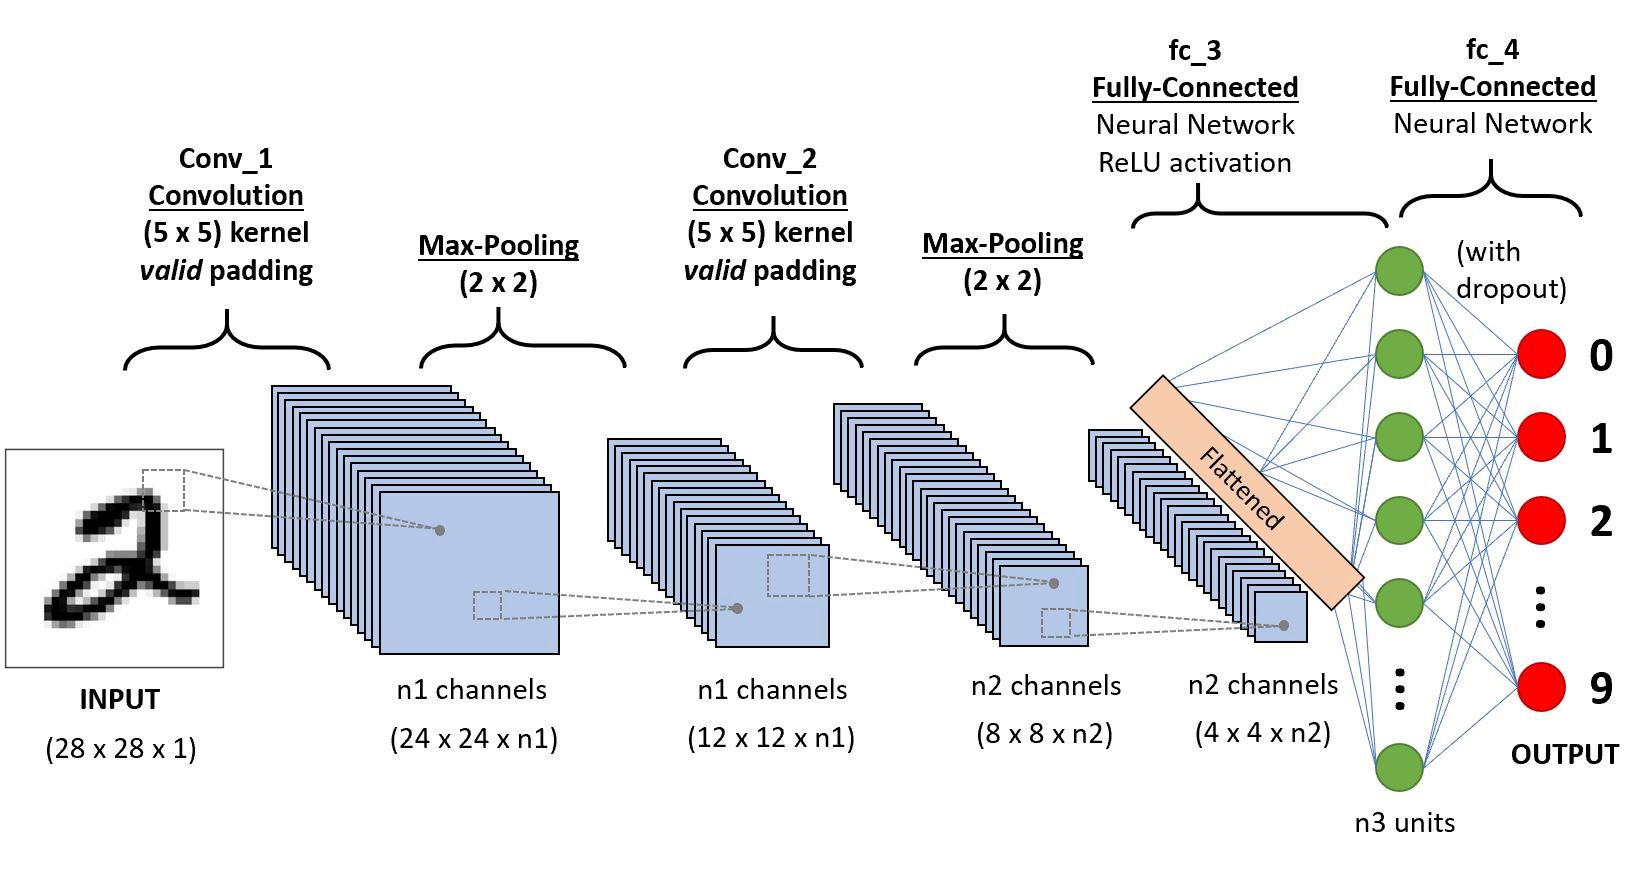
\includegraphics[width=0.9\linewidth]{images/typical-cnn.png}
	\caption{Mạng nơ-ron tích chập điển hình\cite{Ratan_2023}}
	\label{fig:typical-cnn}
\end{figure}

Tổng quan, mạng nơ ron tích chập là một kiến trúc mạng nơ ron đặc biệt được thiết kế để xử lý và trích xuất đặc trưng từ dữ liệu ảnh. Các đặc điểm của CNN như lớp tích chập, lớp gộp, lớp kích hoạt, lớp kết nối đầy đủ và tính chia sẻ tham số giúp cho CNN có khả năng học và trích xuất các đặc trưng từ dữ liệu ảnh một cách hiệu quả. Kiến trúc kiểu "tầng" trong CNN cho phép mạng học được các đặc trưng từ cấp thấp đến cấp cao, từ các nét cơ bản đến các đặc trưng phức tạp hơn.

\subsection{Dữ liệu đầu vào}

Dữ liệu hình ảnh đầu vào cho mạng nơ-ron tích chập (CNN) thường là các bức ảnh được biểu diễn dưới dạng ma trận điểm ảnh. Mỗi điểm ảnh trong ma trận thể hiện mức độ sáng tại mỗi vị trí trên ảnh.

Thông thường các ảnh màu đầu vào sẽ có các kênh màu RGB, trong đó mỗi kênh màu tương ứng với một thành phần màu đỏ (R), xanh lá cây (G) và xanh dương (B). Với mỗi điểm ảnh, giá trị của từng kênh màu (R, G, B) thường được biểu diễn bằng một con số trong khoảng từ 0 đến 255.

Kích thước của ảnh đầu vào có thể khác nhau tùy thuộc vào yêu cầu của bài toán và kiến trúc của mạng CNN. Các kích thước phổ biến cho ảnh đầu vào là 224x224, 256x256, 299x299 hoặc 512x512 điểm ảnh.

Trước khi đưa dữ liệu hình ảnh vào mạng CNN, dữ liệu cần đưa qua một số bước tiền xử lý:

\begin{enumerate}
	\item Chuẩn hóa: Để đảm bảo rằng các giá trị pixel trong ảnh nằm trong khoảng từ 0 đến 1. Như vậy cần phải chuẩn hóa dữ liệu bằng cách chia tất cả các giá trị điểm ảnh cho 255 đối với kiểu dữ liệu 8 bít hoặc chia cho $2^n-1$ với $n$ là kích thước số nguyên của điểm ảnh.
	\item Thay đổi kích thước: Nếu kích thước của ảnh không phù hợp với kích thước đầu vào của mạng CNN, cần thực hiện điều chỉnh kích thước ảnh để phù hợp. Thông thường, sử dụng phép thay đổi tuyến tính hoặc cắt ảnh để thay đổi kích thước ảnh.
	\item Tăng cường dữ liệu huấn luyện: Đối với các bài toán mạng CNN, việc sử dụng kỹ thuật tăng cường dữ liệu khi huấn luyện có thể giúp tăng tính tổng quát hóa của mô hình. Tăng cường dữ liệu bao gồm việc áp dụng các phép biến đổi như xoay, lật, phóng to, thu nhỏ, và thay đổi độ sáng để tạo ra các phiên bản mới của dữ liệu hình ảnh.
\end{enumerate}

Dữ liệu trong cnn được biểu diễn dưới dạng ma trận. Dữ liệu hình ảnh đầu vào sẽ được biểu diễn dưới dạng \ref{input_shape}.

\begin{equation}
	\centering
	\label{input_shape}
	(N \times C \times H_{in} \times W_{in})
\end{equation}

Trong đó
\begin{itemize}
	\item $N$ là số hình ảnh đầu vào theo lô.
	\item $C$ là số kênh, ảnh mức xám có số kênh bằng 1, ảnh RGB có số kênh bằng 3.
	\item $H_{in}$ là chiều cao ảnh.
	\item $W_{in}$ là chiều rộng ảnh.
\end{itemize}

\subsection{Lớp tích chập}

\subsubsection{Phép chập}

Phép chập là một phép toán cơ bản trong xử lý ảnh dùng để xác định đặc trưng giữa các điểm ảnh trong một hình ảnh và xây dựng các bộ lọc để trích xuất đặc trưng hay thực hiện các phép biến đổi hình ảnh. Hình \ref{fig:edge-detection-conv} mô tả ứng dụng của phép tích chập trong bài toán phát hiện biên theo chiều dọc.

% TODO: \usepackage{graphicx} required
\begin{figure}[h]
	\centering
	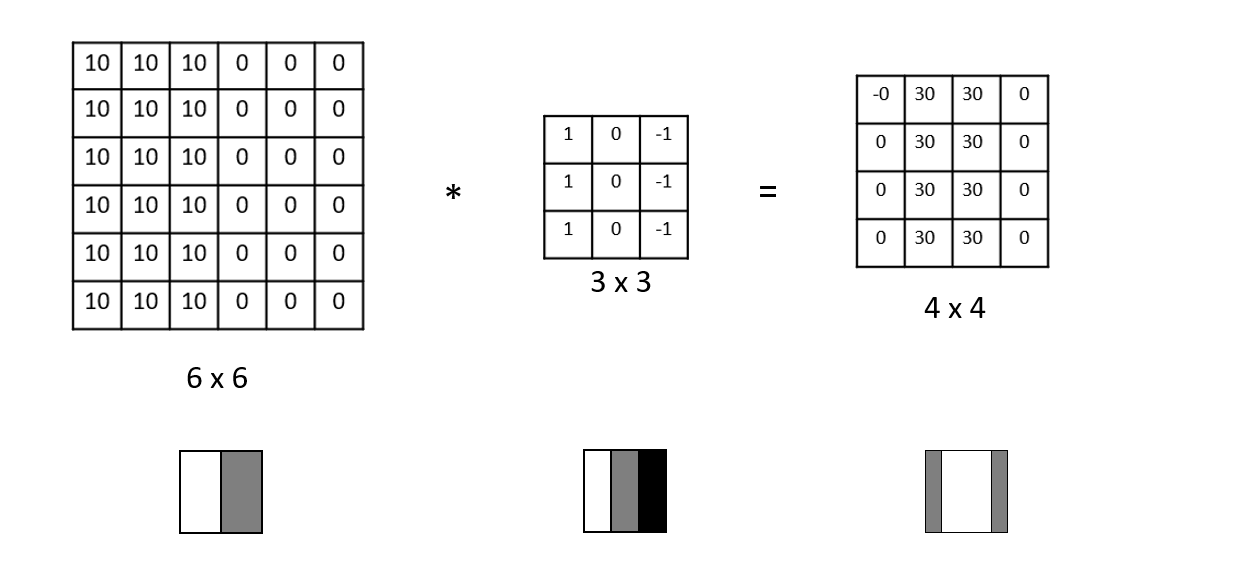
\includegraphics[width=0.8\linewidth]{images/edge-detection-conv}
	\caption{Phép tích chập trong phát hiện dọc}
	\label{fig:edge-detection-conv}
\end{figure}

Bộ lọc hay nhân trong phép tích chập là một ma trận được xoay $180^\circ$, trượt tới từng vị trí của ma trận vào. Kết quả từng vị trí của ma trận kết quả trong phép tích chập tính bằng cách tính tổng của tích từng phần tử của nhân đã được xoay $180^\circ$ với phần tử tại vị trí tương ứng trên ma trận vào. Nói cách khác, kết quả phép chập là kết quả phép tương quan chéo giữa ma trận đầu vào với nhân được xoay $180^\circ$ \ref{eqn:conv-basic}.

\begin{equation}\label{eqn:conv-basic}
	x_{ij} = \sum^{m-1}_{a = 0} \sum^{m-1}_{b = 0} k_{ab} y_{(i+a)(j+b)}, k' = rot180(k)
\end{equation}

Trong thực thế, lớp tích chập trong CNN có thể loại bỏ phép xoay và sử dụng phép tương quan chéo nhằm mục đích tối ưu tích toán mà không ảnh hưởng tới kết quả của mạng \cite{8721631}. Như vậy, thay vì công thức \ref{eqn:conv-basic} lớp tích chạp có thể sử dụng công thức \ref{eqn:correlate-basic} thay thế.

\begin{equation}\label{eqn:correlate-basic}
	x_{ij} = \sum^{m-1}_{a = 0} \sum^{m-1}_{b = 0} k_{ab} y_{(i+a)(j+b)}
\end{equation}

Hình \ref{fig:conv-operation} mô tả quá trình thực hiện chập ma trận vào với bộ lọc để được kết quả phần tử đầu tiên của ma trận ra.

% TODO: \usepackage{graphicx} required
\begin{figure}
	\centering
	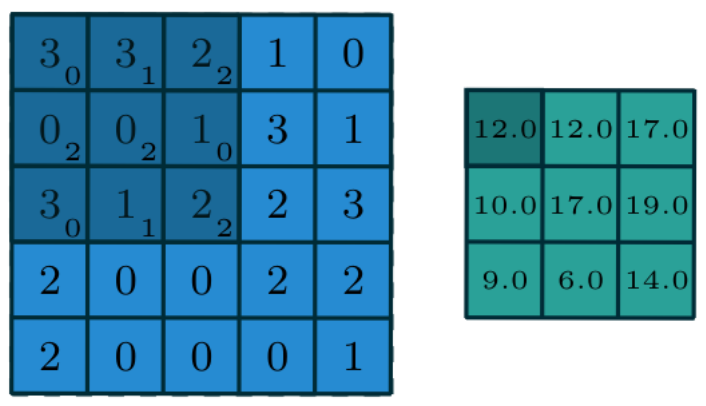
\includegraphics[width=0.6\linewidth]{images/conv-operation}
	\caption{Phép chập}
	\label{fig:conv-operation}
\end{figure}

\subsubsection{Kích thước bộ lọc}

Kích thước bộ lọc $k$ là kích thước của ma trận bộ lọc trong phép tích chập. Trong phần lớn trường hợp, kích thước bộ lọc được sử dụng có dạng vuông, tức chiều rộng bằng chiều cao và bằng $k$. 

Kích thước của bộ lọc có ảnh hưởng đến cách tính toán phép tích chập và kích thước của đầu ra. Khi bộ lọc có kích thước lớn hơn, nó có khả năng nhìn thấy một khu vực lớn hơn trên đầu vào và có thể giúp phát hiện các đặc trưng toàn cục. Tuy nhiên, nó cũng tăng độ phức tạp tính toán và có thể dẫn đến việc mất thông tin chi tiết trong đầu vào. Ngược lại, khi bộ lọc có kích thước nhỏ hơn, nó tập trung vào phát hiện các đặc trưng cục bộ và tạo ra đầu ra có kích thước nhỏ hơn. Các giá trị thông thường cho kích thước bộ lọc là 3\times 3, 5\times 5, 7\times 7.

\subsubsection{Thuộc tính đệm}

Thông thường, khi chập trực tiếp bộ lọc với ma trận vào ta sẽ thu được ma trận ra với kích thước nhỏ hơn (Hình \ref{fig:no-padding-unit-stride}). Do đó,đệm được sử dụng để thay đổi kích thước đầu vào trước khi áp dụng tích chập nhằm thu được đầu ra theo ý muốn.

% TODO: \usepackage{graphicx} required
\begin{figure}[h]
	\centering
	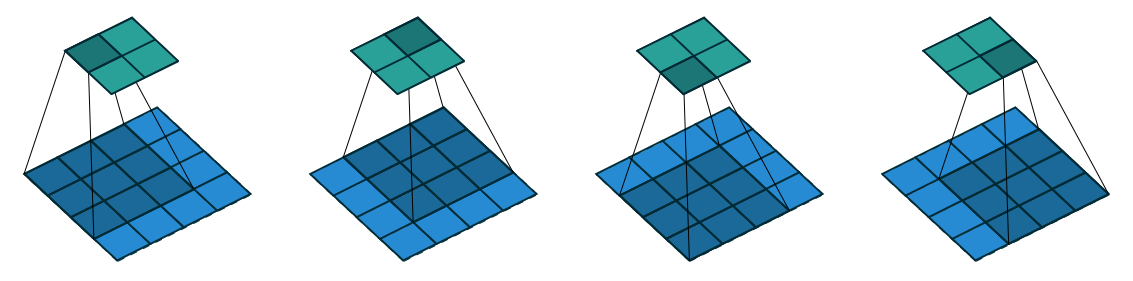
\includegraphics[width=0.9\linewidth]{images/no-padding-unit-stride}
	\caption{Chế độ không đệm, bước nhảy đơn vị}
	\label{fig:no-padding-unit-stride}
\end{figure}

Có 2 loại đệm:
\begin{itemize}
	\item Đệm nửa đảm bảo kích thước ma trận đầu ra bằng kích thước ma trận đầu vào (Hình \ref{fig:half-padding-unit-stride1}). Giá trị đệm nửa xác định bằng công thức \ref{eqn:haft-padding}.
	\begin{equation}\label{eqn:haft-padding}
		p = \frac{k-1}{2}
	\end{equation}
	\item Đệm đầy đủ đảm bảo kích thước ma trận đầu ra lớn hơn hoặc bằng kích thước ma trận đầu vào (Hình \ref{fig:full-padding-unit-stride}). Giá trị đệm đầy đủ tính bằng công thức \ref{eqn:full-padding}.
	\begin{equation}\label{eqn:full-padding}
		p = k-1
	\end{equation}
\end{itemize}
% TODO: \usepackage{graphicx} required
\begin{figure}
	\centering
	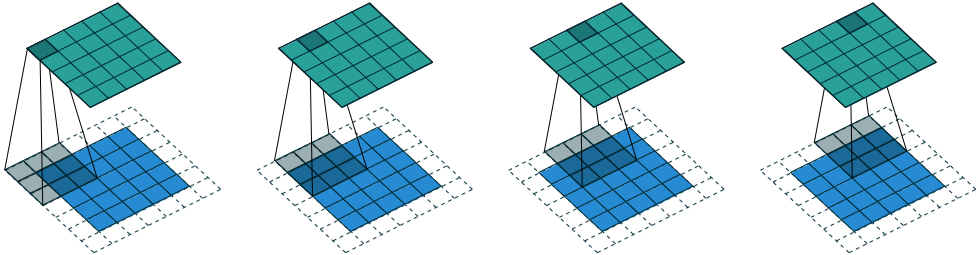
\includegraphics[width=0.9\linewidth]{images/half-padding-unit-stride1}
	\caption{Chế độ đệm nửa, bước nhảy đơn vị}
	\label{fig:half-padding-unit-stride1}
\end{figure}

% TODO: \usepackage{graphicx} required
\begin{figure}
	\centering
	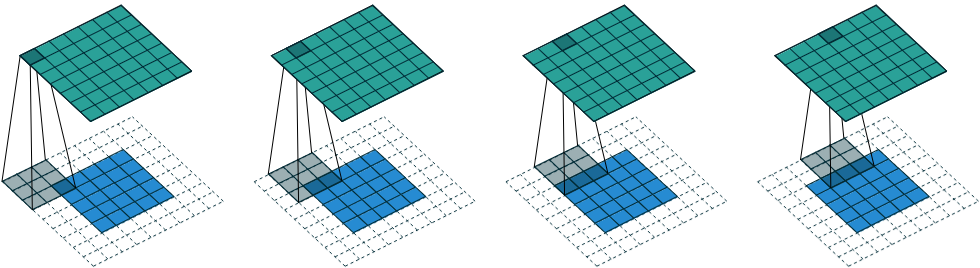
\includegraphics[width=0.9\linewidth]{images/full-padding-unit-stride}
	\caption{Chế độ đệm đầy đủ, bước nhảy đơn vị}
	\label{fig:full-padding-unit-stride}
\end{figure}

\subsubsection{Thuộc tính bước nhảy}

Bước nhảy là số lượng phần tử giữa hai lần áp dụng tích chập ma trận đầu vào với bộ lọc. Như vậy, thay vì di chuyển 1 điểm ảnh trên ảnh đầu vào trong phép tích chập thông thường, áp dụng bước nhảy sẽ di chuyển ma trận với $s$ điểm ảnh (Hình \ref{fig:half-padding-stride-2}).

% TODO: \usepackage{graphicx} required
\begin{figure}[h]
	\centering
	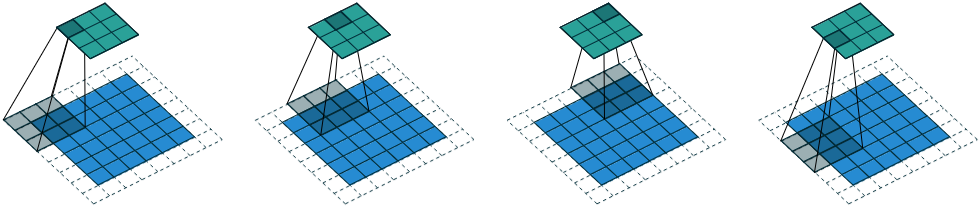
\includegraphics[width=0.9\linewidth]{images/half-padding-stride-2}
	\caption{Chế độ đệm nửa, bước nhảy 2}
	\label{fig:half-padding-stride-2}
\end{figure}

Sử dụng bước nhảy có thể làm giảm kích thước của đầu ra so với đầu vào ban đầu, vì những vị trí không được xem xét. Tuy nhiên, bước nhảy cũng giúp giảm độ phức tạp tính toán và số lượng tham số trong mạng nơ-ron tích chập, đồng thời có thể tạo ra các biểu diễn đặc trưng tổng quát hơn và giảm hiện tượng overfitting.


Việc kết hợp bước nhảy và đệm tạo ra ma trận với kích thước tính theo công thức \ref{eqn:padding-stride}.

\begin{equation}\label{eqn:padding-stride}
	o = \lfloor{\frac{i-k}{s}}\rfloor + 1
\end{equation}

\subsubsection{Phép chập khối}

Trong thực tế, việc áp dụng các bộ lọc trên ảnh thường được áp dụng cho cả 3 kênh màu đỏ, lục và lam. Như vậy, bộ lọc hay khối lọc cần có 3 chiều bao gồm màu sắc, chiều cao và chiều rộng. 

Hình \ref{fig:single-filter-block-conv} mô tả ảnh đầu vào kích thước $6 \times 6$ trên hệ màu RGB. Như vậy, đầu vào có thể biểu diễn dạng ma trận kích thước $(6 \times 6 \times 3)$. Khối lọc để áp dụng tương ứng cũng phải có 3 lớp tương ứng với 3 màu đỏ, lục và lam.

% TODO: \usepackage{graphicx} required
\begin{figure}[h]
	\centering
	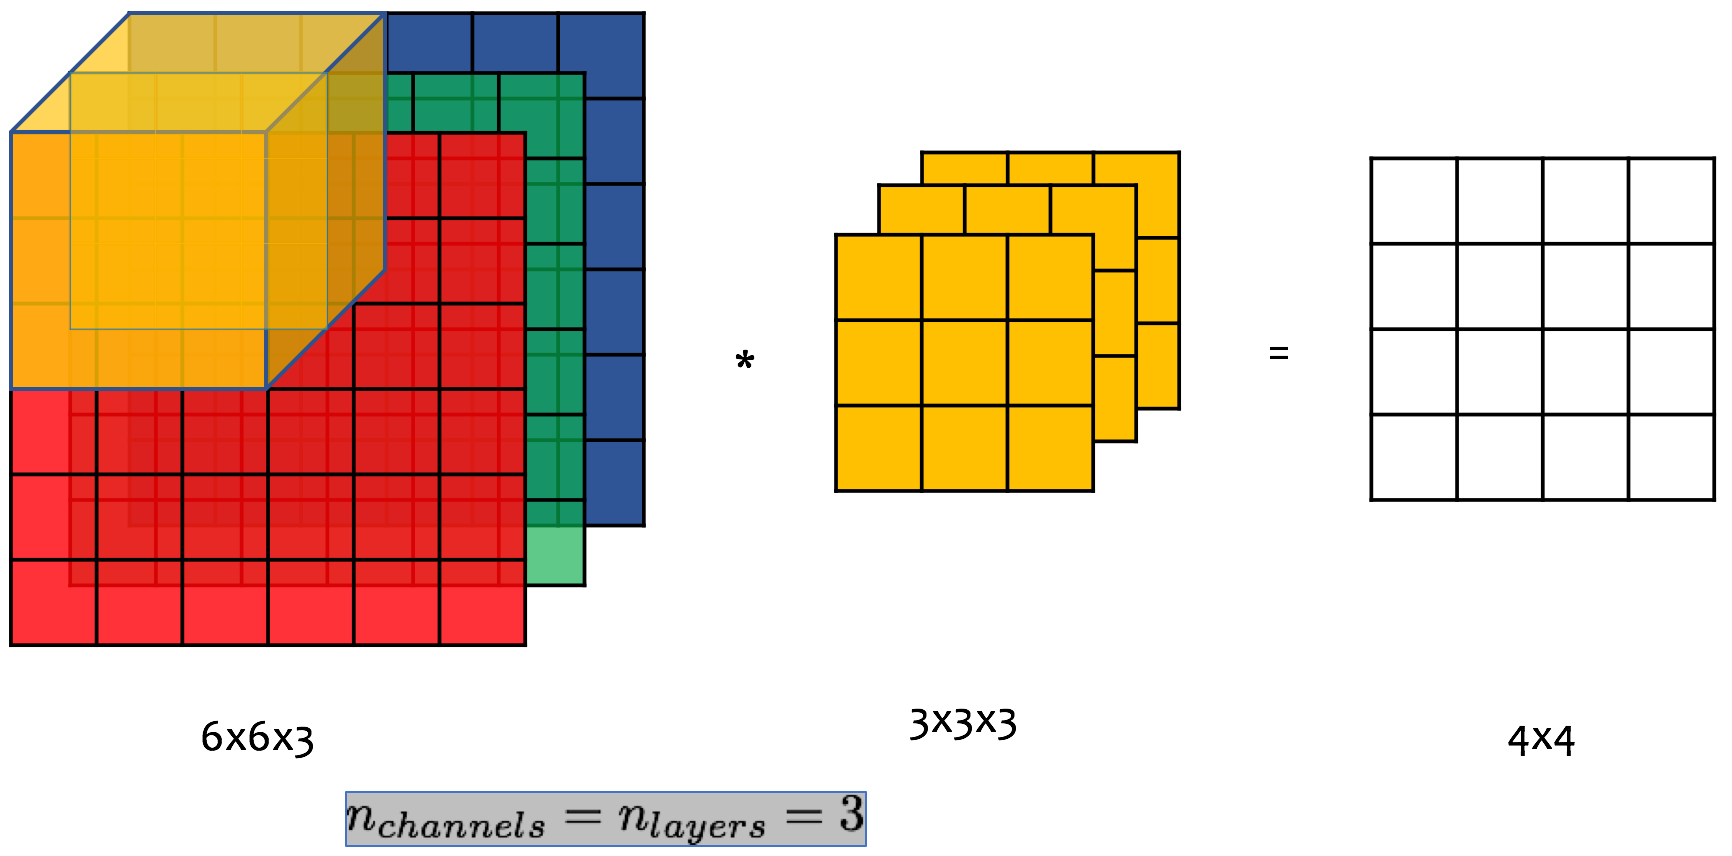
\includegraphics[width=0.8\linewidth]{images/single-filter-block-conv}
	\caption{Phép chập khối \cite{dl_ap_2018}}
	\label{fig:single-filter-block-conv}
\end{figure}

Việc tính toán kết quả sau khi áp dụng khối lọc thực hiện bằng cách dịch chuyển khối lọc trên khối ma trận vào. Mỗi lớp của bộ lọc được chập với diện tích phủ bởi nó trên kênh tương ứng của ma trận vào. Tại một vị trí tương ứng của khối lọc, giá trị tại ô tương ứng của ma trận đầu ra là tổng của các kết quả phép chập trên từng lớp.

Như vậy, dữ liệu đầu vào có thể có nhiều kênh khác nhau, tương ứng với đó, các bộ lọc cũng phải có số kênh tương ứng. Kết quả phép chập giữa ma trận đầu vào $X$ với $n$ kênh và khối lọc $K$ được tính bằng công thức \ref{eqn:block-conv}.

\begin{equation}\label{eqn:block-conv}
	Y = \sum^n_{i=1}X_i\star K_i
\end{equation}

Phép chập có thể được sử dụng để phát hiện và trích xuất đặc trưng trên một hoặc nhiều kênh vào. Ví dụ, để phát hiện đặc trưng trên kênh màu đỏ và bỏ qua kênh màu xanh lục và xanh lam, bộ phát hiện chỉ được đặt ở lớp đầu tiên và giá trị 2 lớp còn lại bằng 0.



\subsubsection{Phép chập khối với nhiều bộ lọc}

Sau mỗi khối lọc, kết quả thu được sau khi thực hiện chập với ma trận khối đầu vào là một ma trận 2 chiều tương ứng với một đặc trưng của đầu vào. Để thu được nhiều đặc trưng từ ảnh đầu vào hay để sinh ra $d$ đặc trưng khác nhau, có thể sử $d$ khối lọc lần lượt chập với ma trận đầu vào để thu được $d$ ma trận đầu ra, xếp chồng chúng trở thành $d$ kênh đầu ra (Hình \ref{fig:multiple-filter-block-conv}).

% TODO: \usepackage{graphicx} required
\begin{figure}[h]
	\centering
	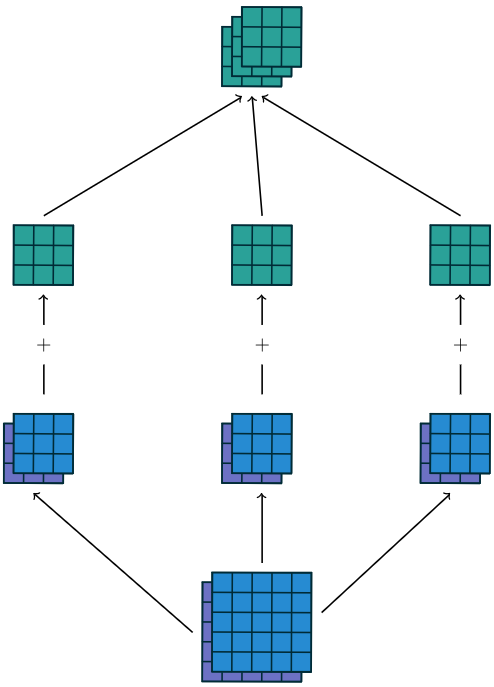
\includegraphics[width=0.6\linewidth]{images/multiple-filter-block-conv}
	\caption{Phép chập nhiều bộ lọc \cite{wei2021}}
	\label{fig:multiple-filter-block-conv}
\end{figure}

Như vậy, thêm vào giá trị hiệu chỉnh $B$ cho từng kênh đầu vào, lớp tích chập có thể được tính tổng quát bằng công thức \ref{eqn:conv-layer}.

\begin{equation}\label{eqn:conv-layer}
	Y_i = B_i + \sum^n_{j=1}X_j \star K_{ij}, i = 1...d 
\end{equation}

\subsection{Lớp gộp}
Lớp gộp là một lớp quan trọng giúp giảm kích thước không gian đầu ra của lớp trước đó trong mạng CNN. 

Mục tiêu chính của lớp gộp là giảm số lượng tham số và tính toán trong mạng nơ-ron, đồng thời giữ lại các đặc trưng quan trọng. Lớp gộp thực hiện điều này bằng cách áp dụng một phép gộp (pooling operation) lên các vùng không gian của đầu vào và trích xuất thông tin quan trọng từ những vùng này.

Có hai loại phép gộp phổ biến trong lớp gộp:

\begin{itemize}
	\item Gộp cực đại: Phép gộp cực đại lấy giá trị lớn nhất trong mỗi vùng không gian của đầu vào. Nó giúp tìm ra đặc trưng nổi bật nhất trong mỗi vùng và giữ lại thông tin quan trọng (Hình \ref{fig:max-pooling}).
	\item Gộp trung bình: Phép gộp trung bình tính giá trị trung bình của các điểm ảnh trong mỗi vùng không gian của đầu vào. Nó có thể giữ lại thông tin tổng quát về mức độ xuất hiện của đặc trưng trong mỗi vùng (Hình \ref{fig:avg-pooling}).
\end{itemize}


% TODO: \usepackage{graphicx} required
\begin{figure}[h]
	\centering
	\begin{subfigure}{.4\textwidth}
		\centering
		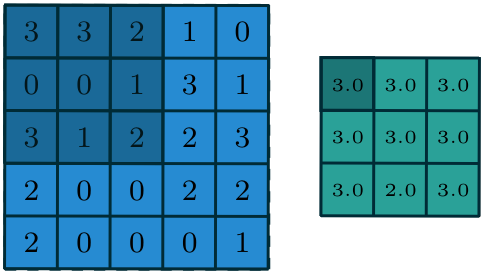
\includegraphics[width=.9\linewidth]{images/max-pooling}
		\caption{Gộp cực đại}
		\label{fig:max-pooling}
	\end{subfigure}

	\begin{subfigure}{.4\textwidth}
		\centering
		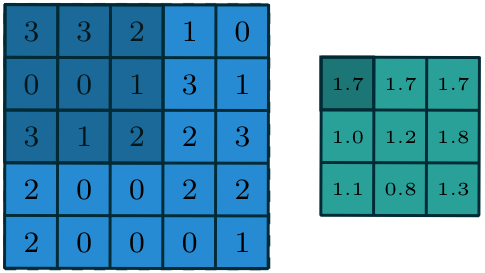
\includegraphics[width=.9\linewidth]{images/avg-pooling}
		\caption{Gộp trung bình}
		\label{fig:avg-pooling}
	\end{subfigure} %
	\caption{Thuật toán gộp cực đại và gộp trung bình với bước nhảy đơn vị}
\end{figure}

Giống như lớp tích chập, lớp gộp cũng có thể sử dụng độ bước nhảy để xác định khoảng cách di chuyển của khung gộp trên ma trận vào. Nếu bước nhảy là 1 hay bước nhảy đơn vị, khung gộp sẽ di chuyển một bước một vị trí trong mỗi lần tính toán. Nếu bước nhảy lớn hơn 1, khung gộp sẽ di chuyển nhanh hơn và kích thước của ma trận kết quả sẽ nhỏ hơn so với đầu vào.

Lớp gộp thường được sử dụng sau mỗi lớp tích chập trong mạng CNN để giảm kích thước không gian của đặc trưng và tổng quát hóa thông tin. Việc giảm kích thước không gian giúp giảm số lượng tham số và tính toán, đồng thời tạo ra các đặc trưng cấp cao hơn bằng cách tóm tắt thông tin từ các vùng lớn hơn của đầu vào.

Tuy nhiên, lớp gộp cũng có một nhược điểm là khiến mất mất một số thông tin chi tiết, vì chỉ giữ lại thông tin quan trọng nhất. Điều này có thể làm mất một số thông tin nhỏ nhưng quan trọng, đặc biệt đối với các bài toán yêu cầu độ chính xác cao.

\subsection{Lớp kích hoạt}
Lớp kích hoạt trong mạng CNN là một lớp không có trọng số và thường được đặt sau mỗi lớp tích chập hoặc lớp kết nối đầy đủ trong mạng.

Nguyên lý hoạt động của lớp kích hoạt như sau:

\begin{itemize}
    \item Đầu vào: Lớp kích hoạt nhận đầu vào từ lớp trước đó trong mạng nơ-ron. Đầu vào có thể là một tensor hoặc một ma trận, tùy thuộc vào kiến trúc của mạng nơ-ron.
    \item Hàm kích hoạt: Lớp kích hoạt áp dụng một hàm kích hoạt phi tuyến tính lên đầu vào. Hàm kích hoạt này thường được chọn để giới hạn đầu ra và tạo độ không tuyến tính cho mạng nơ-ron. Một số hàm kích hoạt phổ biến bao gồm:
    \begin{itemize}
        \item Hàm ReLU (Rectified Linear Unit): $f(x) = max(0, x)$. Nó giữ nguyên giá trị không âm và bỏ qua các giá trị âm.
        \item Hàm Sigmoid: $f(x) = \frac{1}{1 + e^{-x}}$. Nó chuyển đổi giá trị đầu vào thành một phạm vi từ $0$ đến $1$, thường được sử dụng trong các bài toán phân loại nhị phân.
        \item Hàm Tanh: $f(x) = \frac{e^x - e^{-x}}{e^x +x e^{-x}}$. Tương tự như hàm sigmoid, nhưng đầu ra nằm trong khoảng từ $-1$ đến $1$.
        \item Hàm Softmax: $f(x_i) = \frac{e^{x_i}}{\sum^n_j e^{x_j}}$, với $i$ là chỉ số của đầu ra và $j$ là chỉ số của tất cả các đầu ra. Hàm softmax thường được sử dụng trong bài toán phân loại đa lớp để chuyển đổi đầu vào thành các xác suất phân loại.
    
    \end{itemize}
    \item Đầu ra: Kết quả của lớp kích hoạt là đầu ra của lớp này, được truyền tới lớp tiếp theo của mạng.
\end{itemize}
    
Lớp kích hoạt chủ yếu được sử dụng để tạo độ không tuyến tính trong mạng nơ-ron và giúp mô hình học được các đặc trưng phức tạp và biểu diễn các mô hình quan hệ phi tuyến. Nó cũng giúp giới hạn đầu ra trong một phạm vi nhất định và tạo ra các đầu ra dễ hiểu và dễ xử lý cho các lớp tiếp theo.

Các hàm kích hoạt và vị trí của lớp kích hoạt trong mạng nơ-ron có thể được điều chỉnh tùy thuộc vào bài toán cụ thể và kiến trúc mạng nơ-ron.

\subsection{Lớp kết nối đầy đủ}
Lớp kết nối đầy đủ còn được gọi là lớp đầu ra trong mạng nơ-ron, là một trong những loại lớp quan trọng trong kiến trúc mạng nơ-ron truyền thẳng.

Nguyên tắc hoạt động của lớp kết nối đầy đủ như sau:

\begin{itemize}
    \item Đầu vào: Lớp kết nối đầy đủ nhận đầu vào từ lớp trước đó trong mạng nơ-ron. Đầu vào thường là một vector hoặc một tensor được duỗi thành một vector.
    \item Trọng số và độ lệch: Mỗi nút trong lớp kết nối đầy đủ kết nối với tất cả các nút trong lớp trước đó thông qua một trọng số (weight) tương ứng. Mỗi kết nối có một trọng số riêng. Ngoài ra, mỗi nút cũng có một độ lệch (bias) tương ứng.
    \item Tính toán: Đầu vào của mỗi nút trong lớp kết nối đầy đủ được nhân với trọng số tương ứng và cộng với độ lệch. Sau đó, kết quả được đưa qua một hàm kích hoạt phi tuyến tính (như hàm ReLU, sigmoid, tanh) để tạo ra đầu ra của nút đó.
    \item Đầu ra: Kết quả tính toán của mỗi nút trong lớp kết nối đầy đủ là đầu ra của lớp này. Đầu ra có thể là một vector hoặc một tensor tùy thuộc vào số lượng nút trong lớp.
\end{itemize}

Lớp kết nối đầy đủ thường được sử dụng trong các mạng nơ-ron truyền thẳng để tạo ra đầu ra cuối cùng của mạng. Nó giúp mô hình học được các mối quan hệ phức tạp giữa đầu vào và đầu ra. Các lớp kết nối đầy đủ thường được sử dụng trong các bài toán như phân loại ảnh, nhận dạng giọng nói, bài toán dự báo, và nhiều bài toán khác.

Một số kiến trúc mạng nơ-ron sử dụng nhiều lớp kết nối đầy đủ liên tiếp nhau để tạo thành một mạng nơ-ron sâu (deep neural network). Trong các mạng nơ-ron sâu, thông qua việc kết hợp nhiều lớp kết nối đầy đủ với các hàm kích hoạt phi tuyến tính, mô hình có khả năng học được các đặc trưng phức tạp và biểu diễn các mô hình quan hệ phi tuyến giữa đầu vào và đầu ra.


\subsection{Mạng tích chập toàn phần}

Mạng tích chập toàn phần (FCN) được sử dụng rộng rãi trong bài toán xử lý ảnh và phân vùng ảnh. So với CNN truyền thống, FCN không có các lớp kết nối đầy đủ ở cuối mạng mà thay vào đó, FCN chỉ sử dụng các lớp tích chập, lớp gộp và kích hoạt trong mạng (Hình \ref{fig:fcn1}). Trong bài toán phân vùng ảnh, mô hình cần gán nhãn cho từng điểm ảnh trong mỗi vùng (Hình \ref{fig:fcn2}). Từ các vùng ảnh, có thể đánh giá hộp bao cho vật thể trong bài toán phát hiện vật thể.

% TODO: \usepackage{graphicx} required
\begin{figure}[h]
	\centering
	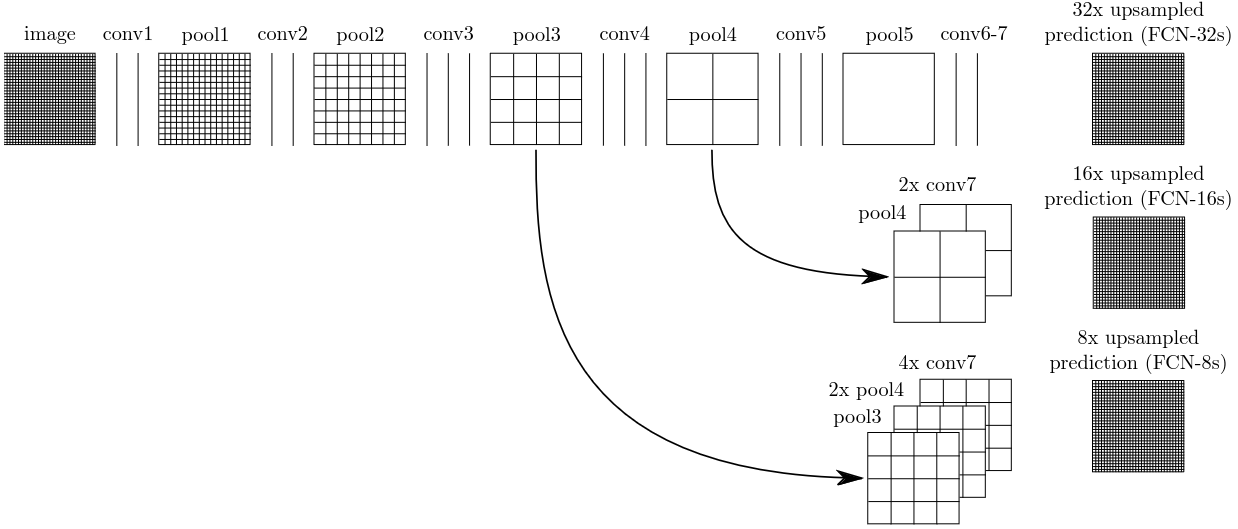
\includegraphics[width=0.99\linewidth]{images/fcn1}
	\caption{Mạng tích chập toàn phần}
	\label{fig:fcn1}
\end{figure}

% TODO: \usepackage{graphicx} required
\begin{figure}[h]
	\centering
	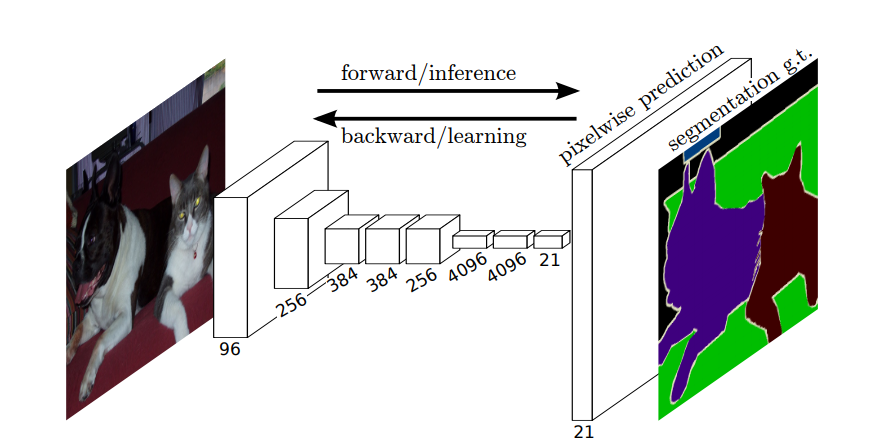
\includegraphics[width=0.9\linewidth]{images/fcn2}
	\caption{Bài toán phân vùng ảnh}
	\label{fig:fcn2}
\end{figure}




\subsection{Mạng đặc trưng kim tự tháp}

Việc phát hiện vật thể trở nên rất thách thức đối với các vật thể nhỏ. Một phương pháp dễ hiểu là sinh đặc trưng với từng tỉ lệ khác nhau như kim tự tháp trên mạng. Tuy nhiên, phương pháp này gây lãng phí tài nguyên tính toán và bộ nhớ. Vì vậy, mạng đặc trưng kim tự tháp (FPN) ra đời với mục tiêu cân bằng giữa độ chính xác và tốc độ xử lý.

FPN bao gồm một đường từ dưới lên và một luồng từ trên xuống. Đường từ dưới lên thực hiện trích xuất đặc trưng. Càng lên cao độ phân giải càng giảm và giá trị thông tin về ngữ cảnh càng cao. Luồng từ trên xuống có chức năng xây dựng các lớp có độ phân giải cao từ các lớp có thông tin ngữ cảnh cao (Hình \ref{fig:fpn}).

% TODO: \usepackage{graphicx} required
\begin{figure}[h]
	\centering
	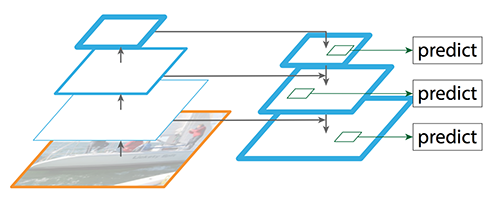
\includegraphics[width=0.8\linewidth]{images/fpn}
	\caption{Mô hình đặc trưng kim tự tháp}
	\label{fig:fpn}
\end{figure}

Trong quá trình xây dựng từ trên xuống, thông tin của đối tượng sẽ bị mất mát. Vì vậy, các kết nối tắt đồng cấp sẽ giúp quá trình dự đoán vị trí các đối tượng tốt hơn, hạn chế tối đa việc mất mát thông tin

\subsection{Hàm mất mát}

Hàm mất mát là một hàm số được sử dụng trong quá trình huấn luyện mô hình máy học để đo lường sự khác biệt giữa các dự đoán của mô hình và giá trị thực tế của dữ liệu đích. Mục tiêu của việc tối ưu hàm mất mát là điều chỉnh các tham số của mô hình để giảm thiểu sai số giữa dự đoán và giá trị thực tế.

Hàm mất mát thường được xây dựng dựa trên mục tiêu cụ thể của vấn đề máy học mà bạn đang giải quyết.

Trong bài toán phát hiện đối tượng, hai hàm mất mát quan trọng nhất là hàm mất mát về lớp đối tượng và hàm mất mát về hộp bao.

Gọi vùng hình ảnh chiếm chỗ thực tế của đối tượng là $A$, vùng hình ảnh dự đoán được của mô hình là $A'$, có thể dễ dàng tính toán được vùng giao và hợp của hai vùng $A$ và $A'$. Hàm mất mát về hộp bao có thể được tính toán từ hai vùng này (Công thức \ref{eqn:iou}).

\begin{equation} 
	\label{eqn:iou}
	IoU=\frac{A\cup A'}{A\cap A'}
\end{equation}

Mọi thay đổi liên quan đến vị trí hoặc hình dạng hộp bao đều làm giảm $IoU$, vì vậy, $IoU$ có thể được sử dụng đánh giá độ chính xác về cả vị trí và hình dạng hộp bao, tối ưu các tham số nhằm sinh $IoU$ cao hơn giúp tăng độ chính xác của mô hình khi xác định hộp bao của vật thể.

Đối với hàm mất mát về lớp đối tượng, hàm mất mát có thể thuộc dạng $1 - 0$, nghĩa là đúng hoặc sai trong dự đoán, hoặc sử dụng phương pháp đo lường sự khác biệt giữa phân phối xác suất dự đoán của mô hình với phân phối xác suất thực tế của các lớp.

Gọi $y_i$ là xác suất của lớp thứ $i$ trong tập dữ liệu, $y'_i$ là xác suất của lớp $i$ trong tập dự đoán, có thể xây dựng hàm mất mát như công thức \ref{eqn:ce-loss}. Như vậy, nếu xác suất dự đoán chính xác càng thấp, giá trị mất mát càng nhỏ và ngược lại.

\begin{equation}
	\label{eqn:ce-loss}
	L_{CE} = - \sum_{i = 1}^{n}y_ilog(y'_i)
\end{equation}

\subsection{Quá trình lan truyền thuận}

Quá trình lan truyền thuận là quá trình dữ liệu được đưa vào qua lớp đầu vào. Các trọng số và hệ số điều chỉnh của mạng được sử dụng để tính toán giá trị đầu ra của mỗi nơ-ron trong lớp tiếp theo.

Trong CNN với nhiều lớp tích chập, đầu ra của các lớp tích chập được đưa vào hàm kích hoạt phi tuyến tính trước khi làm đầu vào cho các lớp tiếp theo. Như vậy, kết quả của lớp tích chập \ref{eqn:conv-layer} sẽ được đưa vào hàm kích hoạt trước khi làm đầu vào cho các tầng tiếp theo. 

Đầu ra của lớp tích chập cuối cùng có thể được xử lý để đưa ra kết quả của mạng với đầu vào tương ứng hoặc được đưa vào các mạng tiếp theo để phục vụ mục đích bài toán như phân loại, ...



\subsection{Quá trình lan truyền nghịch}
Trong quá trình huấn luyện mạng, từ kết quả của quá trình lan truyền thuận, có thể xác định được sự chênh lệch về kết quả đoán nhận được so với kết quả thực tế. Quá trình lan truyền nghịch được sử dụng để tinh chỉnh giá trị trọng số trong các nhân lớp tích chập và hệ số tinh chỉnh tương ứng. 

Độ lệch trong số $\omega_{ab}$ có thể tính theo công thức \ref{eqn:back-prop1}.

\begin{equation}\label{eqn:back-prop}
	\frac{dE}{dw_{ab}} = \sum^{N-m}_{i=0}\sum^{N-m}_{j=0} \frac{dE}{dx^l_{ij}} \frac{dx^l_{ij}}{d\omega_{ab}} =  \sum^{N-m}_{i=0}\sum^{N-m}_{j=0} \frac{dE}{dx^l_{ij}} y^{l-1}_{(i+a)(j+b)}
\end{equation}

Độ dốc $\frac{dE}{dx^l_{ij}}$ được tính bằng công thức \ref{eqn:back-prop2}:
\begin{equation}\label{eqn:back-prop2}
	\frac{dE}{dx^l_{ij}} = \frac{dE}{dy^l_{ij}}\frac{dy^l_{ij}}{dx^l_{ij}} =  \frac{dE}{dy^l_{ij}} \frac{d}{dx^l_{ij}}(\sigma (x^l_{ij})) = \frac{dE}{dy^l_{ij}}\sigma' ((x^l_{ij}))
\end{equation}

Ngoài các giá trị trọng số phải tính hiện tại, quá trình huấn luyện còn cần biết độ thay đổi của tham sô đầu vào lớp hiện tại để tiếp tục áp dụng cho các lớp trước đó. Độ thay đổi được tính bằng công thức \ref{eqn:back-prop3}.

\begin{equation}\label{eqn:back-prop3}
	\frac{dE}{dy^{l-1}_{ij}} = \sum^{m-1}_{a=0} \sum^{m-1}_{b=0} \frac{dE}{dx^l_{(i-a)(j-b)}} \frac{dx^l_{(i-a)(j-b)}}{dy^{l-1}_{ij}} = \sum^{m-1}_{a=0} \sum^{m-1}_{b=0} \frac{dE}{dx^l_{(i-a)(j-b)}}\omega_{ab}
\end{equation}

\subsection{Đánh giá hiệu suất của mạng nơ-ron tích chập}
Trong mạng nơ-ron tích chập (CNN), có một số thông số quan trọng được sử dụng để đánh giá hiệu suất của mô hình:
\begin{itemize}
	\item  Độ chính xác $Accuracy$ là tỷ lệ phần trăm của số lượng dự đoán chính xác trên tổng số lượng dự đoán. Độ chính xác được tính bằng công thức \ref{eqn-acc}.
	\begin{equation}
		\label{eqn:acc}
		Accuracy = \frac{TP + TN}{TP + TN + FP + FN}
	\end{equation}
	
	\item Độ chính xác dương tính $Precision$ đo lường tỷ lệ giữa số lượng dự đoán dương tính chính xác và tổng số lượng dự đoán dương tính. Đây là tỉ lệ giữa số lượng dự đoán "đúng" chính xác và tổng số lượng dự đoán "đúng" (Công thức \ref{eqn:prec}).
	\begin{equation}
		\label{eqn:prec}
		Precision = \frac{TP}{TP + FP}
	\end{equation}	
	\item Độ nhớ tìm kiếm $Recall$ còn được gọi là độ nhạy, đo lường tỷ lệ giữa số lượng dự đoán dương tính chính xác và tổng số lượng thực tế dương tính. Đây là tỉ lệ giữa số lượng dự đoán "đúng" chính xác và tổng số lượng dự đoán "đúng" thực tế.
	\begin{equation}
		\label{eqn:recall}
		Recall = \frac{TP}{TP + FN}
	\end{equation}	
	
	\item Điểm F1 là một đánh giá tổng hợp, kết hợp giữa Độ chính xác dương tính và độ nhạy. Nó đo lường sự cân bằng giữa độ chính xác dương tính và độ nhạy. 
	\begin{equation}
		\label{eqn:f1}
		F1_{score} = \frac{2 * (Precision * Recall)}{(Precision + Recall)}
	\end{equation}
	
\end{itemize}


\section{Mô hình YOLO}

\subsection{Giới thiệu mô hình}

Mô hình YOLO là một mô hình phổ biến trong lĩnh vực nhận diện đối tượng và phát hiện vị trí đối tượng trong ảnh và video. Mô hình YOLO có khả năng phân loại và định vị các đối tượng trong một khung hình duy nhất một cách nhanh chóng và chính xác.

Các đặc điểm chính của mô hình YOLO bao gồm:
\begin{itemize}
    \item Kiến trúc: Mô hình YOLO sử dụng mạng nơ-ron tích chập (CNN) để trích xuất đặc trưng từ ảnh đầu vào và dự đoán các hộp giới hạn\ và các lớp đối tượng tương ứng. Kiến trúc gốc của YOLO được gọi là YOLOv1 và sau đó đã có các phiên bản cải tiến như YOLOv2, YOLOv3,  YOLOv4, YOLOv5, YOLOv8, ...
    \item Grid cells: Mô hình YOLO chia ảnh thành một lưới ô vuông có kích thước cố định. Mỗi ô vuông trong lưới được gọi là một grid cell. Mỗi grid cell sẽ dự đoán một số lượng hộp giới hạn và lớp đối tượng tương ứng.
    \item Dự đoán hộp giới hạn: Mỗi grid cell trong mô hình YOLO dự đoán các hộp giới hạn bằng cách dùng các tỷ lệ (scales). Mỗi hộp giới hạn được biểu diễn bằng các thông số như tọa độ (x, y) của trung tâm, chiều rộng và chiều cao của hộp.
    \item Dự đoán lớp đối tượng: Mô hình YOLO dự đoán lớp đối tượng của mỗi hộp giới hạn bằng cách sử dụng softmax trên các điểm đặc trưng (feature points) của ảnh.
    \item Non-max suppression: Sau khi mô hình YOLO đã dự đoán các hộp giới hạn và lớp đối tượng, một quá trình gọi là non-max suppression được áp dụng để loại bỏ các hộp giới hạn trùng lặp và giữ lại các hộp giới hạn có xác suất dự đoán cao nhất.
\end{itemize}


\subsection{Kiến trúc mạng của mô hình}

Kiến trúc mạng YOLO (You Only Look Once) đã trải qua nhiều phiên bản và cải tiến, bao gồm YOLOv1, YOLOv2, YOLOv3 đến YOLOv8. Tuy nhiên, YOLO hiện nay bao gồm các thành phần chính như: Backbone, Neck và Head.

\begin{itemize}
    \item Backbone network: YOLO sử dụng một mạng nơ-ron tích chập (CNN) làm cơ sở để trích xuất đặc trưng từ ảnh. Mạng nền (backbone network) trong YOLO có thể được xây dựng bằng cách sử dụng các kiến trúc như Darknet hoặc CSPDarknet.
    \item Neck: YOLO có một phần gọi là neck (cổ), được đặt giữa backbone network và head của mô hình. Neck có nhiệm vụ kết hợp các đặc trưng từ các tầng khác nhau của feature pyramid để cung cấp thông tin phong phú hơn cho việc dự đoán đối tượng.
    \item Head: Đây là phần cuối cùng của mô hình YOLO, nơi các hộp giới hạn và lớp đối tượng được dự đoán. Head của YOLO sử dụng các lớp tích chập để dự đoán tọa độ và lớp của các hộp giới hạn. Đồng thời, YOLO sử dụng các kỹ thuật như SPP (Spatial Pyramid Pooling) và PANet (Path Aggregation Network) để cải thiện khả năng phát hiện và định vị đối tượng.
\end{itemize}

Với hàm mất mát, mô hình YOLO sử dụng một hàm mất mát kết hợp giữa các thành phần như localization loss, confidence loss và class loss. Hàm mất mát này giúp tối ưu hóa mô hình và cải thiện độ chính xác của các dự đoán.

\subsection{Đánh giá hiệu suất của mô hình}

Qua các phiên bản, mô hình YOLO ngày càng được cải thiện. Hình \ref{fig:yolov8-better} cho thấy các phiên bản YOLO ngày càng được cải thiện với lượng tham số nhỏ hơn nhanh hơn nhưng hiệu suất lại cao hơn.

\begin{figure}
    \centering
    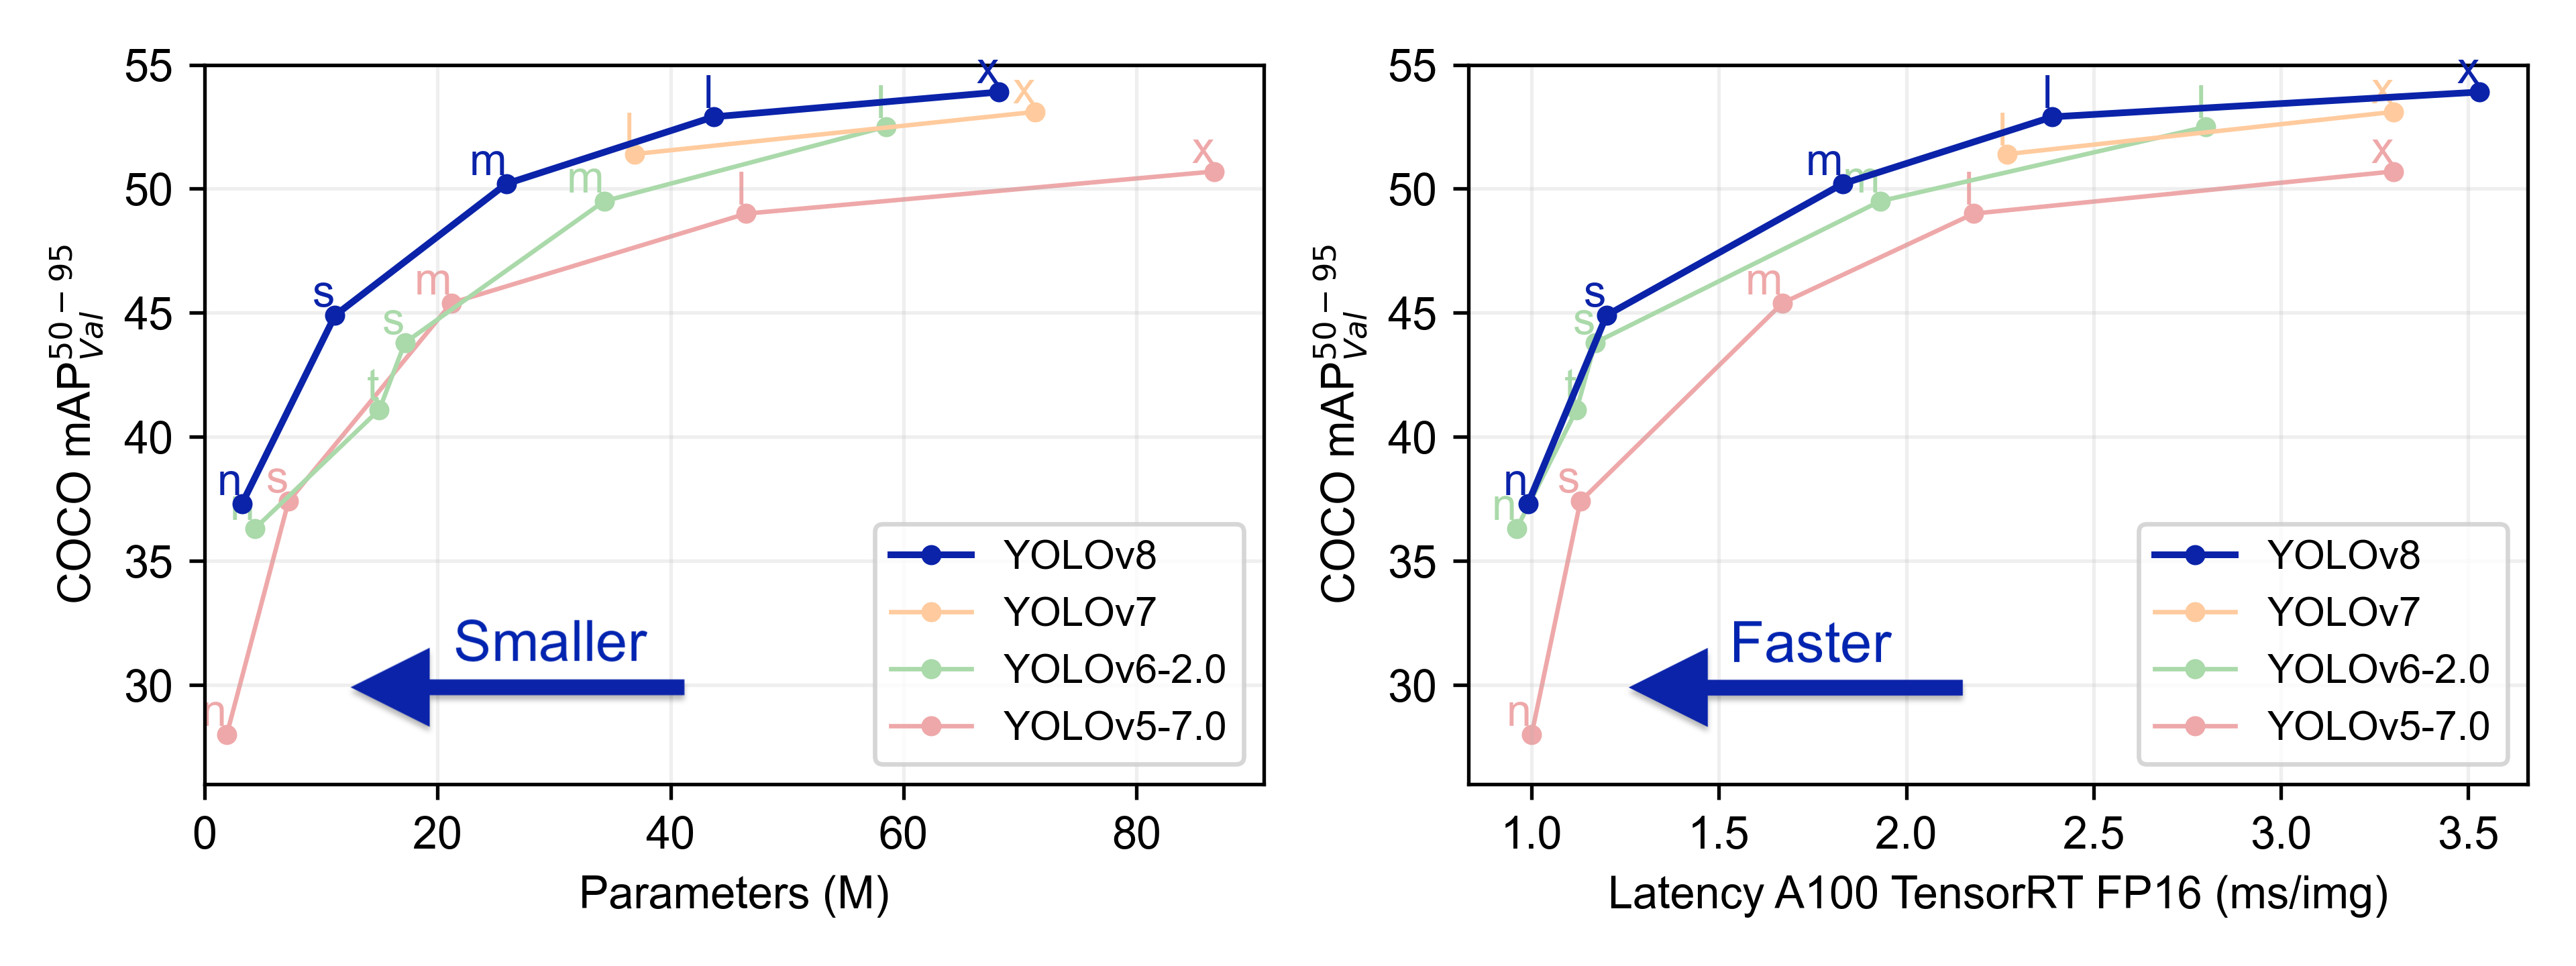
\includegraphics[width=0.75\linewidth]{images/yolov8-better.png}
    \caption{yolov8-better}
    \label{fig:yolov8-better}
\end{figure}
\subsection{So sánh YOLO và CNN trong nhận diện và phân loại ảnh}


\subsubsection{Kiến trúc mạng}
CNN là một kiến trúc mạng nơ-ron sử dụng các tầng tích chập và tầng kết nối đầy đủ để học các đặc trưng của ảnh. CNN thường sử dụng một số tầng tích chập để trích xuất đặc trưng và sau đó sử dụng các tầng kết nối đầy đủ để phân loại ảnh.

YOLO là một kiến trúc mạng nơ-ron đặc biệt được thiết kế cho việc phát hiện và định vị đối tượng trong ảnh. YOLO chia ảnh thành các lưới (grid) và dự đoán các hộp giới hạn (bounding box) và lớp đối tượng cho mỗi lưới. YOLO sử dụng một kiến trúc mạng nơ-ron tích chập để trích xuất đặc trưng và dự đoán đồng thời các hộp giới hạn và lớp đối tượng.

\subsubsection{Tốc độ}

Với CNN, việc phân loại và nhận dạng đối tượng được thực hiện trong các lớp cuối cùng của mạng. Điều này có nghĩa là CNN phải đi qua toàn bộ hình ảnh để đưa ra dự đoán, do đó, tốc độ của CNN thường chậm hơn so với YOLO.

YOLO sử dụng một phương pháp "You Only Look Once" để dự đoán đồng thời các hộp giới hạn và lớp đối tượng trên toàn bộ ảnh. Điều này giúp YOLO có tốc độ rất nhanh, vì nó không cần phải xem xét ảnh nhiều lần.

\subsubsection{Độ chính xác}

Với việc sử dụng các tầng tích chập và kết nối đầy đủ, CNN có thể học các đặc trưng phức tạp từ ảnh và đạt được độ chính xác cao trong các tác vụ phân loại và nhận dạng ảnh.

YOLO có thể cung cấp độ chính xác tương đối cao trong việc phát hiện và định vị đối tượng trong ảnh. Tuy nhiên, do việc dự đoán đồng thời trên toàn bộ ảnh, YOLO có xu hướng không chính xác hơn trong việc định vị các đối tượng nhỏ hoặc gần nhau.

\section{Nghiên cứu ứng dụng CNN và YOLO trong hệ thống theo dõi và chăm sóc nấm}

Với độ chính xác tương đối cao với tác vụ phân loại vật thể và khả năng xác định vùng bao vật thể, mô hình YOLO có thể ứng dụng trong hệ thống theo dõi và chăm sóc nấm. Bằng việc xây dựng bộ dữ liệu với các loại nấm cùng giai đoạn phát triển khác nhau, mô hình có thể cho ra biết vị trí, thời gian và giai đoạn phát triển hiện tại, giúp người nông dân đưa ra quyết định kịp thời hoặc có thể hỗ trợ điều khiển robot tự động làm việc chăm sóc hay chuẩn bị,  thu hoạch nấm.

\section{Hướng phát triển và nâng cao hiệu suất mô hình CNN và YOLO}

Đối với mô hình YOLOv8, mô hình có thể được điều chỉnh với các kích thước khác nhau (Hình \ref{fig:yolov8-structure}).

\begin{figure}
    \centering
    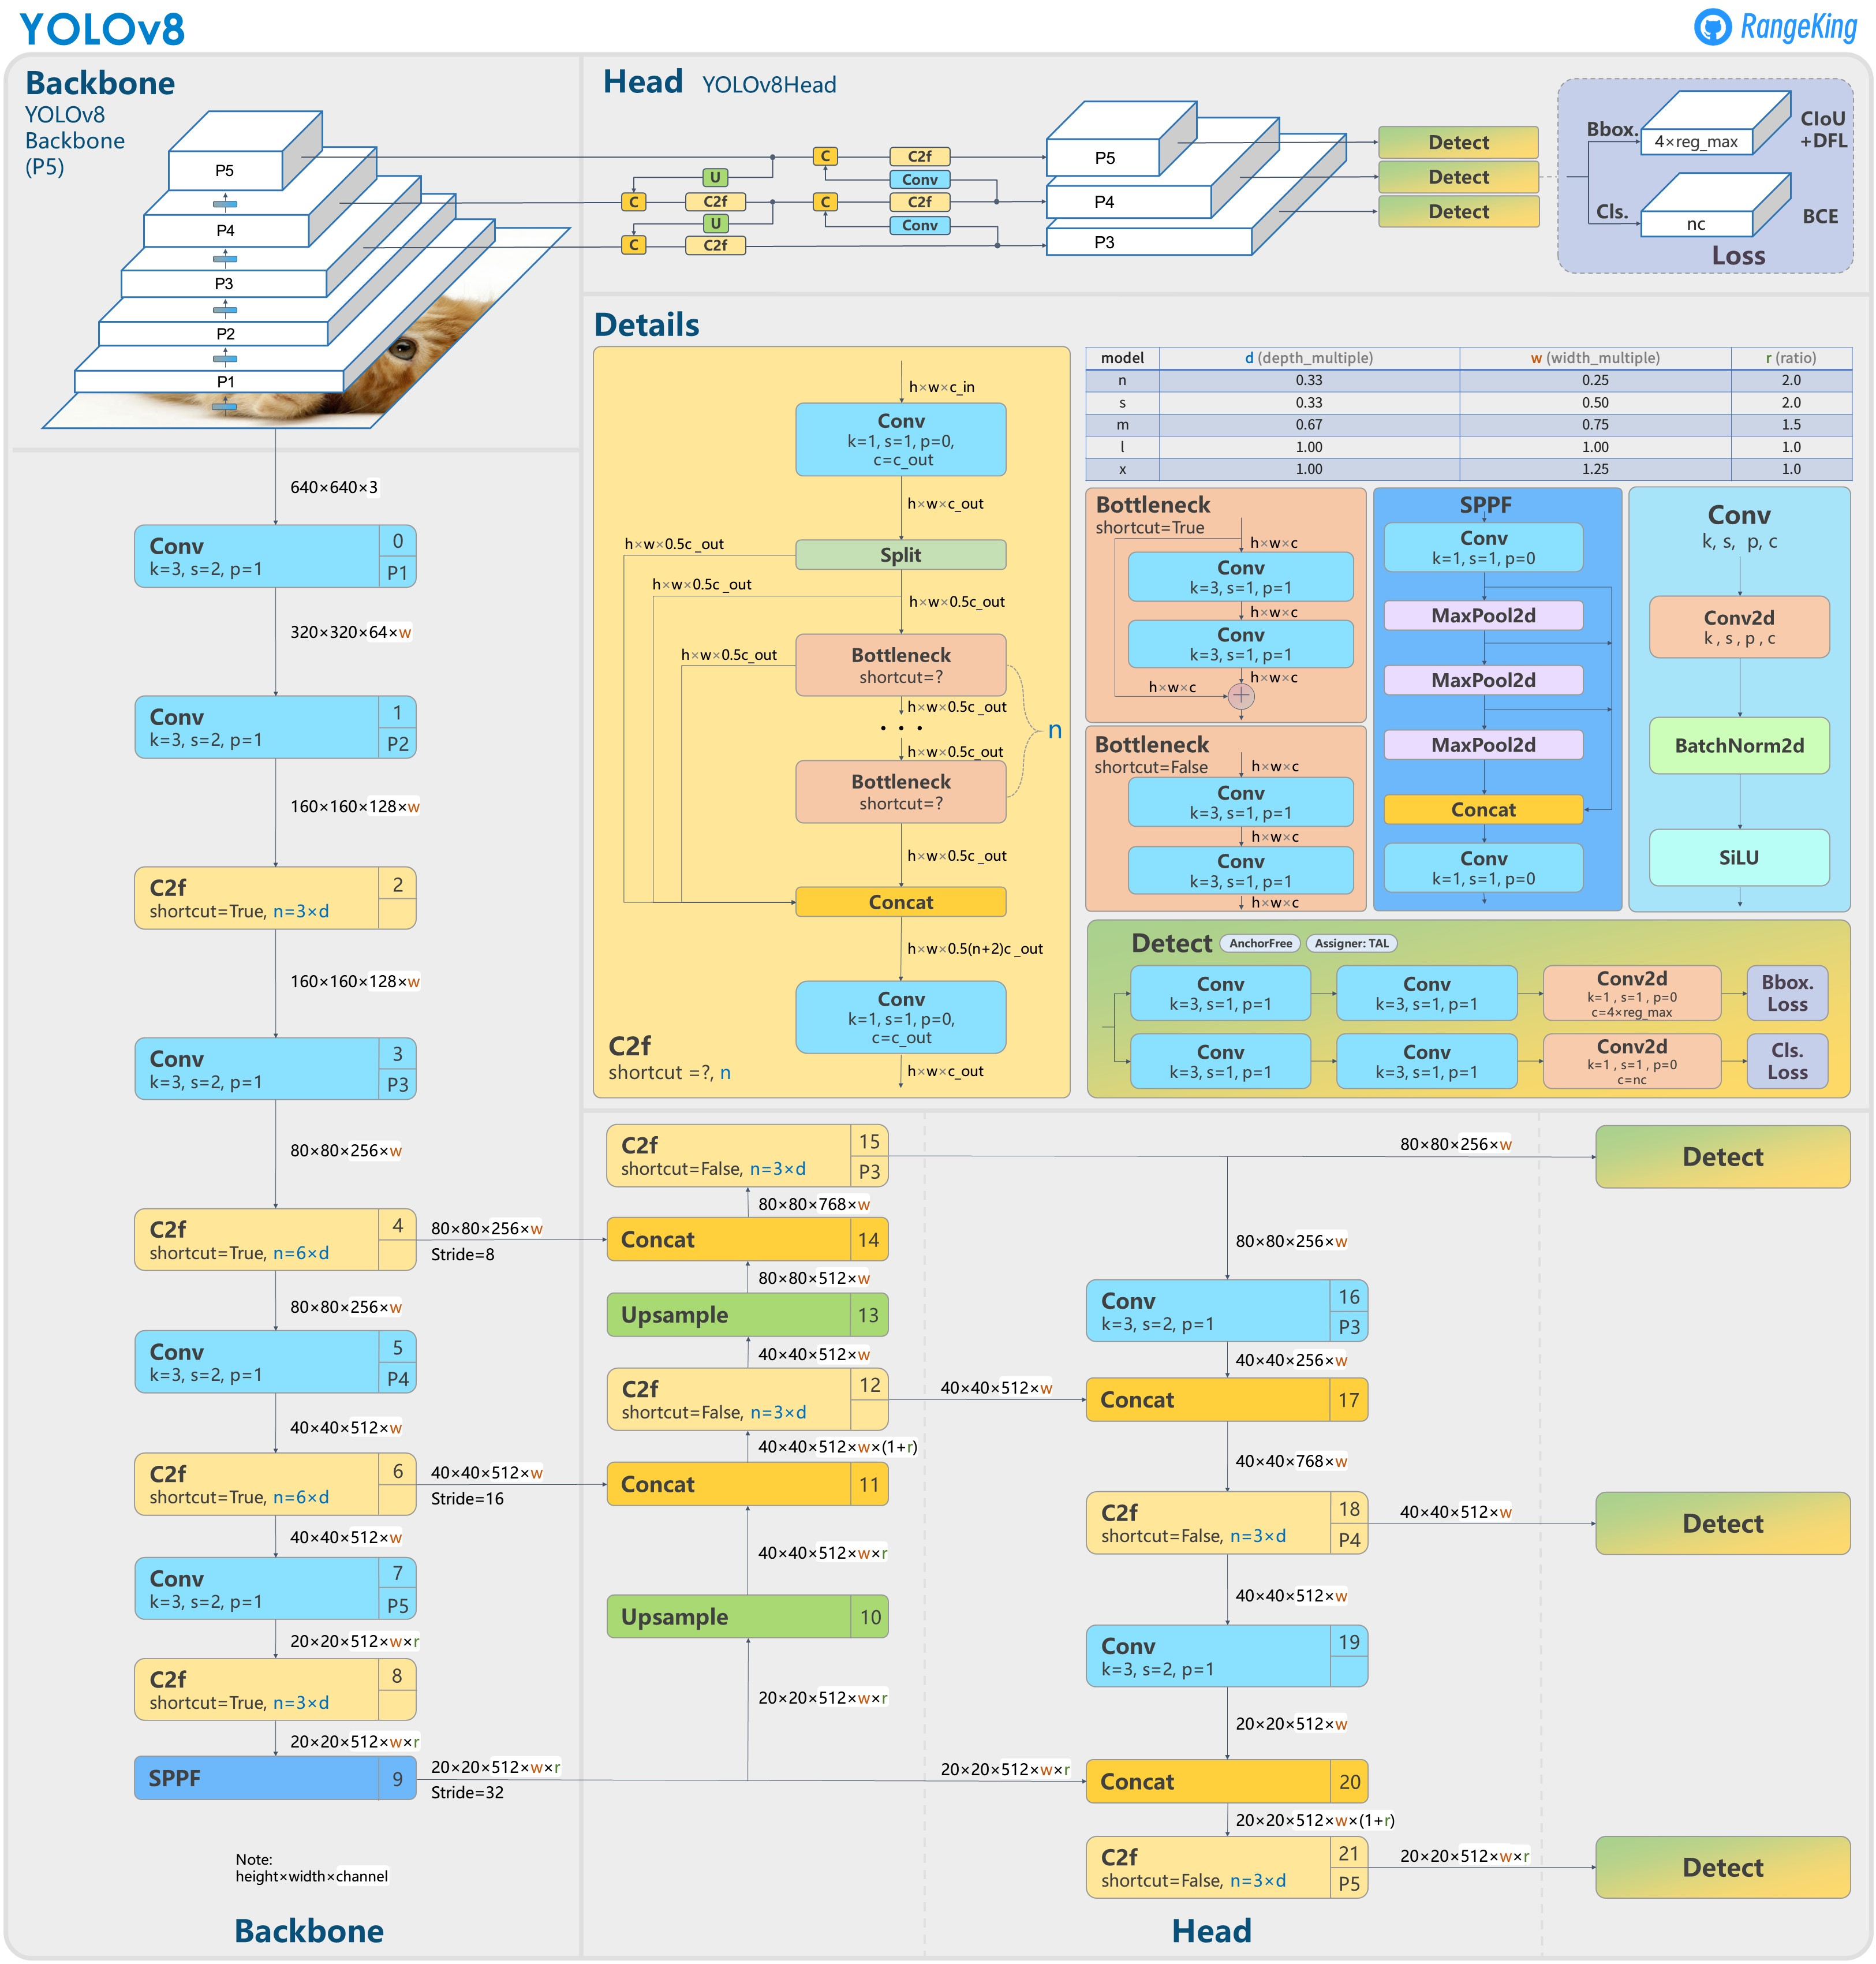
\includegraphics[width=1\linewidth]{images/yolov8-network.png}
    \caption{Cấu trúc mạng YOLOv8 và cấu hình kích thước}
    \label{fig:yolov8-structure}
\end{figure}

Với kích thước lớn - L, mô hình có khả năng học sâu hơn và đưa ra kết quả chính xác hơn. Tuy nhiên, dữ liệu đầu vào cần đa dạng và số lượng lớn hơn để có thể lấy ra những đặc trưng một cách chung nhất. Đối với số lượng mẫu nhỏ, để tránh tình trạng overfitting, kích thước nhỏ như s, n sẽ phù hợp hơn.

\section{Tổng kết chương}


Chương 2 tập trung nghiên cứu ứng dụng của mạng nơ-ron tích chập và mô hình YOLO trong hệ thống theo dõi và chăm sóc nấm.

Trước tiên, mạng nơ-ron tích chập là một mô hình học sâu được thiết kế đặc biệt cho việc xử lý dữ liệu hình ảnh. Nguyên lý hoạt động mạng dựa trên phép tích chập để lấy ra đặc trưng của ảnh, từ đó có thể phân loại ảnh vào các lớp khác nhau.

Tiếp theo, YOLO là một mô hình phát hiện và định vị đối tượng trong ảnh. Với việc chia ảnh thành các ô lưới và dự đoán hộp giới hạn và xác suất cho các đối tượng trong mỗi ô lưới, YOLO mang lại khả năng phát hiện đối tượng nhanh chóng và chính xác.

Cuối cùng là khả năng áp dụng YOLO vào hệ thống giám sát và chăm sóc nấm. Bằng việc phát hiện giai đoạn phát triển và vị trí của nấm, các công việc phân tích, chăm sóc có thể được thực hiện kịp thời. Ngoài ra, chương 2 còn để cập đến hướng phát triển và nâng cao hiệu suất của mô hình CNN và YOLO.

Như vậy, có thể thấy rằng CNN và YOLO có thể được ứng dụng trong hệ thống theo dõi và chăm sóc nấm. Sử dụng các phương pháp này, quá trình phân loại, phát hiện và định vị nấm có thể được tự động hóa, giúp tăng hiệu suất và chính xác, đồng thời giảm công sức và chi phí nhân công.
